\begin{savequote}[75mm]
Going to space shouldn't be like pooping pineapples.
\qauthor{Elon Musk}
\end{savequote}

\chapter{The Cost of Access to Space}
\label{costofaccess}
\begin{multicols*}{2}
\lettrine{W}{ith} advances in launcher technology, the cost of access to space is decreasing rapidly. New innovations in partial-reusability, and the emergence of commercial space -- SpaceX, Orbital Sciences, Blue Origin and Virgin Galactic, to name a few -- is uprooting the traditional conservatism of the space industry. The `Billionaire Race', as it is labelled, is providing a driving force for the shakedown of the `Old Space' community. Aided by the arrival of Moore's Law to the space industry, in the form of nano- and pico-satellites, many space companies are exploiting the use of multiple low-cost satellites to provide the functions of larger, more expensive platforms. %Closer to home, the United Kingdom specialises in the manufacture of small satellites (< 1 tonne), and has provided systems for commercial and governmental entities for a range of mission destinations.

\begin{table}[h]
\centering
\begin{tabular}{cccc}
\toprule
\toprule
Ariane 5 & Falcon 9 & Falcon Heavy \footnotemark & Vega \\
\midrule
10500 & 4100 & 2500 & 15600 \\ 
\bottomrule
\bottomrule
\end{tabular}
\caption{Cost of launch to Low-Earth Orbit, in USD/kg. \citep{Vicens2016}}
\label{t:costofaccess}
\end{table}
\footnotetext{Yet to fly.}
Despite the dramatic reductions in space cost, it is rare that payloads are injected into their final orbit by their launch vehicle. Mission designers are posed with an optimisation problem for every trajectory and mission plan they undertake; that is, the arrival and maintaining of the spacecraft at its' nominal orbit for the least amount of propellant mass. In the case of space missions, which often end when their available propellant is expended, the minimisation of propellant usage is of utmost importance. 

The language of mission designers is not without the perpetual usage of the term $\Delta V$: the overall velocity -- and thus propellant -- required to undertake a maneouvre. 

Konstantin Tsiolkovsky first determined the relationship between velocity increments and propellant mass in 1903, which became one of the most famous and widely-used equations in rocket science, relating the velocity increment $\Delta V$ to the exhaust velocity $v_e$ and the ratio of initial to final masses \citep{Curtis2009}:

\begin{equation}
\Delta v = v_{e}~\textnormal{ln} \bigg( \frac{m_0}{m_f} \bigg)
\label{rocketequation}
\end{equation}

\begin{figure*}[ht]
\centering
\begin{subfigure}{.45\textwidth}
\centering
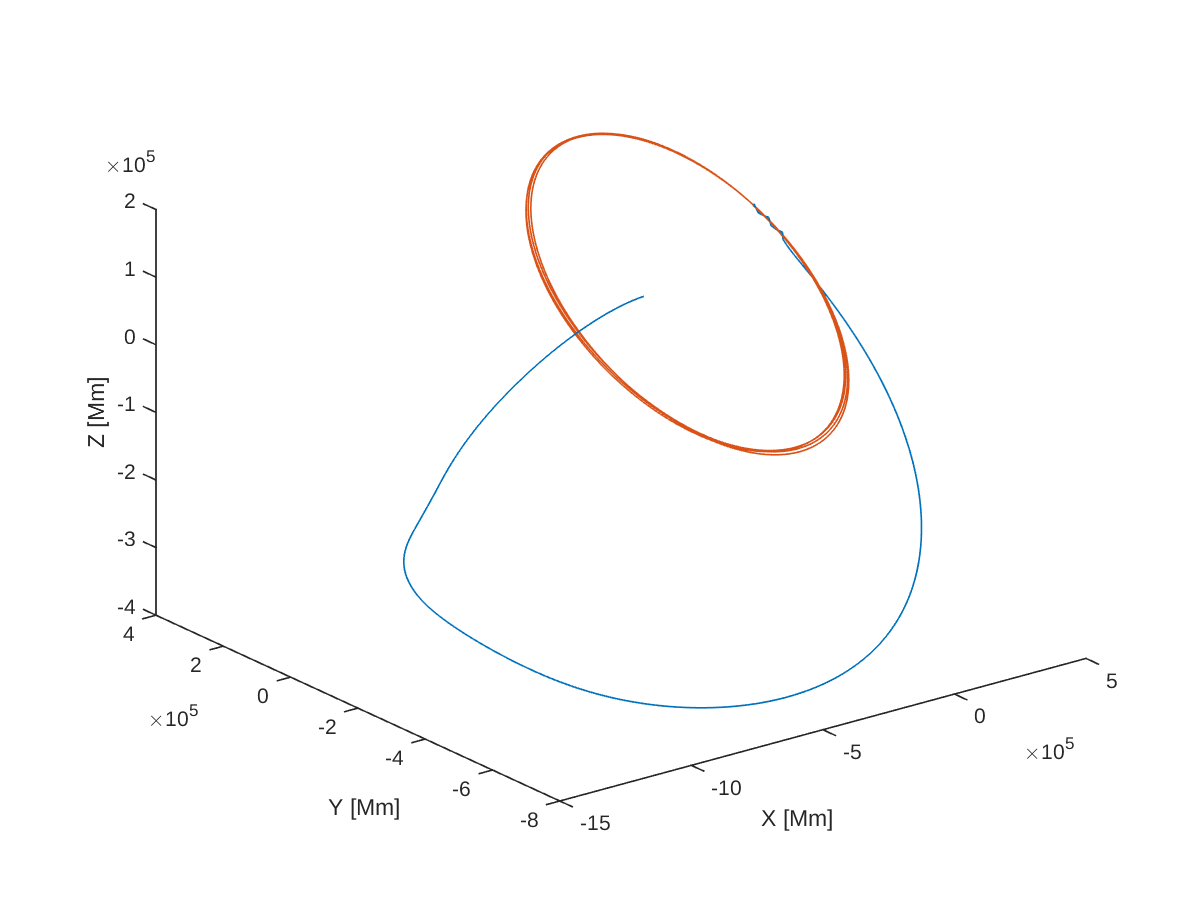
\includegraphics[width=\linewidth]{figures/grail_orbit}
\end{subfigure}%
\begin{subfigure}{.45\textwidth}
\centering
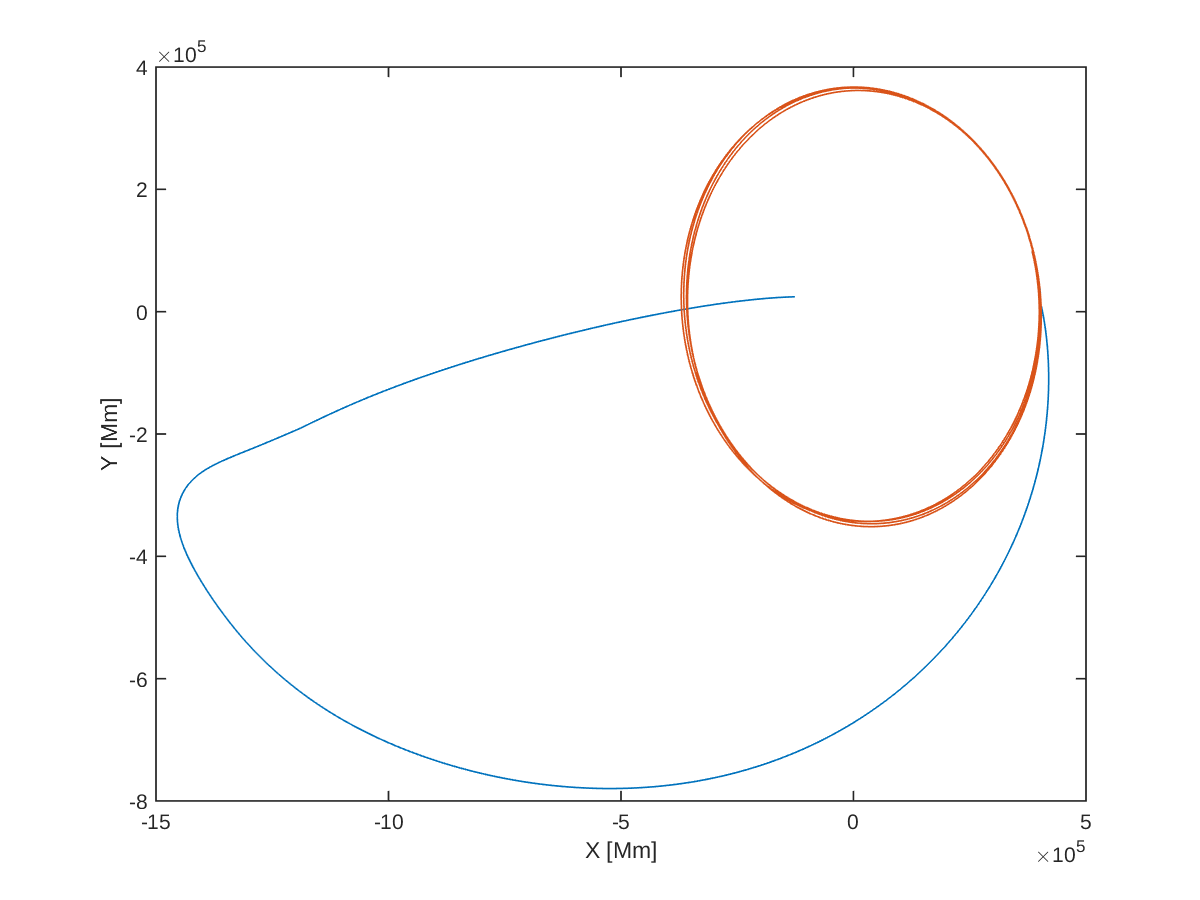
\includegraphics[width=\linewidth]{figures/grail_orbit3}
\end{subfigure}
\caption{The transfer trajectory of NASA's GRAIL spacecraft in the ICRF/J2000 frame. Ephemeris supplied by JPL.}
\label{f:grail}
\end{figure*}

Equation \ref{rocketequation} is the most important equation of all in mission design. Its' tyranny -- a term coined for its' logarithmic nature in increasing $\Delta v$ -- places large limits on attainable destinations in the solar system, and gravity assists from planetary bodies are often required to reach the corners of the solar system with any useful payload mass remaining.

The optimisation problem brought on by Equation \ref{rocketequation} has led to the advent of many techniques for the reduction of propellant mass in space mission design. Perhaps one of those given most attention is the prospect of the \textit{low-energy transfer}. A \textit{low-energy transfer} utilises far less propellant than a more traditional transfer, such as a Hohmann or bi-elliptic transfer, but often at the cost of transit times. Further, the computation of these transfers and trajectories can be delicate, and often exist as a complex harmony of gravitation and chaos. 

The first mission to undertake such a transfer was \textit{Hiten}, a Japanese probe launched to the vicinity of the Moon in 1990. Originally named MUSES-A, its' daughter payload experienced a failure upon injection into Lunar orbit. \citep{Belbruno1993} devised a new method of transfer -- the \textit{weak stability transfer} -- that would allow for injection of MUSES-A, now renamed \textit{Hiten}, into Lunar orbit itself. While a lengthy transit time of five months was present, the capture into Lunar orbit required zero $\Delta v$, and allowed for the transfer to be conducted by the probe's on-board thrusters.

Further exploitation of these types of transfers followed, with NASA's GRAIL satellite utilising an exterior weak-stability transfer to transit to the Moon (Figure \ref{f:grail}. The European Space Agency's SMART-1 mission employed an interior weak-stability transfers to transit to the Moon using low-thrust.

These \textit{low-energy transfers} are the offspring of the applications of dynamical systems theory to space mission design. A particular case of orbital motion, the three-body problem, yields many dynamical structures - stable and unstable manifolds and bounding surfaces - that provide phase-space structures for the transfer of objects into and from the smaller primary body. The use of these dynamical phenomena can provide advantages to the mission designer for dramatic propellant savings.

% The study of the three-body problems and its' dynamical structures can lead to the discovery of \textit{Lagrangian points}, areas in space where the gravitational influences of the two primaries sum to effectively zero, and the spacecraft becomes trapped in what is known as a `halo orbit', a non-Keplerian orbit that oscillates about a particular Lagrange point. 

% The \textit{Lagrangian points} have attracted the attention of mission designers of a range of missions, including Gaia, THEMIS, the Herschel Space Observatory, and the James Webb Space Telescope. These orbital destinations can provide full views of the Sun at the L1 point, and ideal imaging environments at L2.


The following work acts as an introduction to the application of dynamical systems theory to space mission design. Section \ref{s:threebodyproblem} provides a brief introduction to the three-body problem, and includes a derivation from the Newtonian $n$-body problem. A small understanding of orbit theory is assumed, and the Section goes on to cover the zero-velocity curves and forbidden regions of the three-body problem, and its' pseudo-potential and integral of motion, the Jacobi constant. Section \ref{s:numericalintro} lays out an introduction to the numerical methods and techniques used to design and construct orbits in the three-body problem, including Po\'incar\'e maps, single- and multiple-shooting, and numerical integration. From this, we construct an example halo orbit, and use it to introduce the concept of Stable Manifolds. These phenomena are further analysed and formally introduced in Section \ref{s:manifoldintroduction}. The exploitation of these phenomena follows in Section \ref{s:manifoldorbits}.



\end{multicols*}